\documentclass[../main.tex]{subfiles}


\begin{document}

\chapter{Modeling, Numerical Methods, and Problem Solving}

\label{cha:cha3}


\begin{center}
\Large{\textbf{CHAPTER OBJECTIVES}}
\end{center}

\normalsize{The primary objective of this chapter is to provide you with a concrete idea of what
numerical methods are and how they relate to engineering and scientific problem
solving. Specific objectives and topics covered are}

\begin{itemize}

\item Learning how mathematical models can be formulated on the basis of scientific

principles to simulate the behavior of a simple physical system.
\item Understanding how numerical methods afford a means to generate solutions in a
manner that can be implemented on a digital computer.

\item Understanding the different types of conservation laws that lie beneath the models
used in the various engineering disciplines and appreciating the difference
between steady-state and dynamic solutions of these models.

\item Learning about the different types of numerical methods we will cover in this
book.

\end{itemize}
\Large{YOU'VE GOT A PROBLEM}


\normalsize{Suppose that a bungee-jumping company hires you. You're given the task of predicting the velocity of a jumper (Fig. 1.1)  as a function of time during the free-fall part
of the jump. This information will be used as part of a larger analysis to determine the
length and required strength of the bungee cord for jumpers of different mass.
You know from your studies of physics that the acceleration should be equal to the ratio
of the force to the mass (Newton's second law). Based on this insight and your knowledge of physics and fluid mechanics, you develop the following mathematical model for the rate
of change of velocity with respect to time, }
\newpage


    
\begin{wrapfigure}{l}{0.25\textwidth}
    \centering
    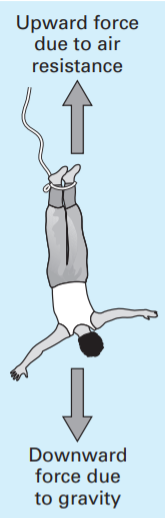
\includegraphics[width=0.25\textwidth]{fig_1_1}
   \caption{\textsf{Forces acting on a free-falling bungee jumper}}
   \label{fig:fig_1_1}
\end{wrapfigure}



$\dfrac{dv}{dt}=g-\dfrac{c_d}{m}v^2$
where $v =$ downward vertical velocity (m/s), $t =$ time (s), $g =$ the acceleration due to
gravity ($\cong$ 9.81 m/s2), $c_d = a$ lumped drag coefficient (kg/m), and $m =$ the jumper's
mass (kg). The drag coefficient is called "lumped" because its magnitude depends on factors such as the jumper's area and the fluid density (see Sec 1.4).


Because this is a differential equation, you know that calculus might be used to obtain
an analytical or exact solution for $v$ as a function of $t$. However, in the following pages, we
will illustrate an alternative solution approach. This will involve developing a computeroriented numerical or approximate solution.


Aside from showing you how the computer can be used to solve this particular problem, our more general objective will be to illustrate (a) what numerical methods are and
(b) how they figure in engineering and scientific problem solving. In so doing, we will also
show how mathematical models figure prominently in the way engineers and scientists use
numerical methods in their work.


\bigskip
\section{A SIMPLE MATHEMATICAL MODEL}
\label{sec:sec1}
  A \textsl{mathematical model} can be broadly defined as a formulation or equation that expresses
the essential features of a physical system or process in mathematical terms. In a very general sense, it can be represented as a functional relationship of the form


\begin{equation}
\tag{1.1}
\overset{Dependent}{variable} = f \left( \overset{independent}{variables},parameters,\overset{forcing}{functions}\right)  
\end{equation}
 
where the \textsl{dependent variable} is a characteristic that typically reflects the behavior or state
of the system; the independent variables are usually dimensions, such as time and space,
along which the system's behavior is being determined; the parameters are reflective of the
system's properties or composition; and the forcing functions are external influences acting
upon it.

The actual mathematical expression of Eq. (1.1) can range from a simple algebraic
relationship to large complicated sets of differential equations. For example, on the basis of
his observations, Newton formulated his second law of motion, which states that the time
rate of change of momentum of a body is equal to the resultant force acting on it. The mathematical expression, or model, of the second law is the well-known equation

\begin{equation}
\tag{1.2}
F=ma
\end{equation}

where $F$ is the net force acting on the body $(N, or kg m/s^2
), m$ is the mass of the object (kg),
and a is its acceleration $(m/s^2
)$.

The second law can be recast in the format of Eq. (1.1) by merely dividing both sides
by $m$ to give
\begin{equation}
\tag{1.3}
a=\dfrac{F}{m}
\end{equation}

where $a$ is the dependent variable reflecting the system's behavior, $F$ is the forcing function, and $m$ is a parameter. Note that for this simple case there is no independent variable
because we are not yet predicting how acceleration varies in time or space.

\begin{itemize}
\item  It describes a natural process or system in mathematical terms.
\item It represents an idealization and simplification of reality. That is, the model ignores negligible details of the natural process and focuses on its essential manifestations. Thus,
the second law does not include the effects of relativity that are of minimal importance
when applied to objects and forces that interact on or about the earth's surface at velocities and on scales visible to humans.
\item  Finally, it yields reproducible results and, consequently, can be used for predictive purposes. For example, if the force on an object and its mass are known, Eq. (1.3) can be
used to compute acceleration.

\end{itemize}


Because of its simple algebraic form, the solution of Eq. (1.2) was obtained easily.
However, other mathematical models of physical phenomena may be much more complex,
and either cannot be solved exactly or require more sophisticated mathematical techniques
than simple algebra for their solution. To illustrate a more complex model of this kind,
Newton's second law can be used to determine the terminal velocity of a free-falling body
near the earth's surface. Our falling body will be a bungee jumper (Fig. 1.1). For this case,
a model can be derived by expressing the acceleration as the time rate of change of the
velocity $(dv/dt)$ and substituting it into Eq. (1.3) to yield

\begin{equation}
\tag{1.4}
\dfrac{dv}{dt}=\dfrac{F}{m}
\end{equation}
where $v$ is velocity (in meters per second). Thus, the rate of change of the velocity is equal
to the net force acting on the body normalized to its mass. If the net force is positive, the
object will accelerate. If it is negative, the object will decelerate. If the net force is zero, the
object's velocity will remain at a constant level.


Next, we will express the net force in terms of measurable variables and parameters.
For a body falling within the vicinity of the earth, the net force is composed of two opposing forces: the downward pull of gravity $F_D$ and the upward force of air resistance $F_U$
(Fig. 1.1):

\begin{equation}
\tag{1.5}
F= F_D + F_U
\end{equation}

If force in the downward direction is assigned a positive sign, the second law can be
used to formulate the force due to gravity as

\begin{equation}
\tag{1.6}
F_D=mg
\end{equation}
where g is the acceleration due to gravity $(9.81 m/s^2
)$.

Air resistance can be formulated in a variety of ways. Knowledge from the science of
fluid mechanics suggests that a good first approximation would be to assume that it is proportional to the square of the velocity,

\begin{equation}
\tag{1.7}
F_U=-c_dv^2
\end{equation}

where $c_d$ is a proportionality constant called the \textsl{lumped drag coefficient} (kg/m). Thus, the
greater the fall velocity, the greater the upward force due to air resistance. The parameter
$c_d$ accounts for properties of the falling object, such as shape or surface roughness, that affect air resistance. For the present case, $c_d$ might be a function of the type of clothing or the
orientation used by the jumper during free fall.
The net force is the difference between the downward and upward force. Therefore,
Eqs. (1.4) through (1.7) can be combined to yield
\begin{equation}
\tag{1.8}
\dfrac{dv}{dt}=g-\dfrac{C_d}{m}v^2
\end{equation}

Equation (1.8) is a model that relates the acceleration of a falling object to the forces
acting on it. It is a \textsl{differential equation} because it is written in terms of the differential rate
of change $(dv/dt)$ of the variable that we are interested in predicting. However, in contrast
to the solution of Newton's second law in Eq. (1.3), the exact solution of Eq. (1.8) for the
velocity of the jumper cannot be obtained using simple algebraic manipulation. Rather,
more advanced techniques such as those of calculus must be applied to obtain an exact or
analytical solution. For example, if the jumper is initially at rest $(v = 0 at t = 0)$, calculus
can be used to solve Eq. (1.8) for

\begin{equation}
\tag{1.9}
v(t)=\sqrt{\dfrac{gm}{c_d}}tanh \left(\sqrt{\dfrac{gc_d}{m}t}\right)
\end{equation}
where tanh is the hyperbolic tangent that can be either computed directly\footnote{{}MATLAB allows direct calculation of the hyperbolic tangent via the built-in function $tanh(x)$.} or via the more
elementary exponential function as in

\begin{equation}
\tag{1.10}
tanhx=\dfrac{e^x-e^{-x}}{e^x+e^{-x}}
\end{equation}

Note that Eq. (1.9) is cast in the general form of Eq. (1.1) where $v(t)$ is the dependent
variable, $t$ is the independent variable, $c_d$ and $m$ are parameters, and $g$ is the forcing function.


\bigskip
\section*{EXAMPLE 1.1. Analytical Solution to the Bungee Jumper Problem }
\label{sec:sec3}
\textbf{Problem Statement.} A bungee jumper with a mass of 68.1 kg leaps from a stationary hot
air balloon. Use Eq. (1.9) to compute velocity for the first 12 s of free fall. Also determine
the terminal velocity that will be attained for an infinitely long cord (or alternatively, the
jumpmaster is having a particularly bad day!). Use a drag coefficient of 0.25 kg/m.

\textbf{Solution.} Inserting the parameters into Eq. (1.9) yields

$$ 
v(t) =\sqrt{\dfrac{9.81(68.1)}{0.25}}tanh \left(\sqrt{\dfrac{9.81(0.25)}{68.1}}t\right)= 51.6938 tanh(0.18977t)
$$
\newpage
which can be used to compute

\begin{figure}[H]
	\centering
	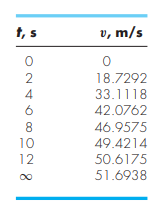
\includegraphics[width=0.25\textwidth]{fig_1_1s}
   \label{fig:fig_1_1s}
\end{figure}



According to the model, the jumper accelerates rapidly (Fig. 1.2). A velocity of
49.4214 m/s (about 110 mi/hr) is attained after 10 s. Note also that after a sufficiently long

\begin{figure}[H]
	\centering
	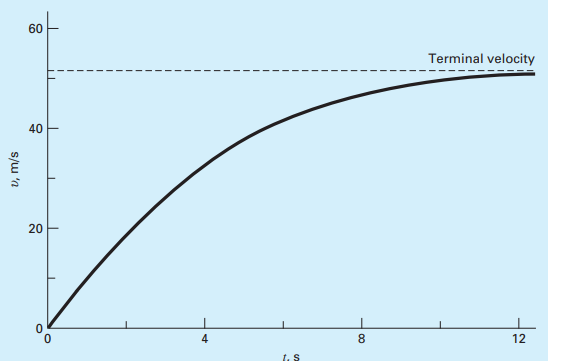
\includegraphics[width=0.75\textwidth]{fig_1_2}
   \caption{\textsf{The analytical solution for the bungee jumper problem as computed in Example 1.1. Velocity
increases with time and asymptotically approaches a terminal velocity.}}
   \label{fig:fig_1_2}
\end{figure}

time, a constant velocity, called the terminal velocity, of 51.6983 m/s (115.6 mi/hr) is
reached. This velocity is constant because, eventually, the force of gravity will be in balance with the air resistance. Thus, the net force is zero and acceleration has ceased.


Equation (1.9) is called an analytical or closed-form solution because it exactly satisfies the original differential equation. Unfortunately, there are many mathematical models
that cannot be solved exactly. In many of these cases, the only alternative is to develop a
numerical solution that approximates the exact solution.
\textit{Numerical methods} are those in which the mathematical problem is reformulated so it
can be solved by arithmetic operations. This can be illustrated for Eq. (1.8) by realizing that
the time rate of change of velocity can be approximated by (Fig. 1.3):

\begin{equation}
\tag{1.11}
\dfrac{dv}{dt}\cong\dfrac{\Delta v}{\Delta t} = \dfrac{v(t_{i+1})-v(t_i)}{t_{i+1}-t_i}
\end{equation}

where $\Delta v$ and $\Delta t$ are differences in velocity and time computed over finite intervals, $v(t_i)$
is velocity at an initial time $t_i$, and $v(t_{i+1})$ is velocity at some later time $(t_{i+1})$. Note that
$dv/dt \cong \Delta v / \Delta t$ is approximate because $ \Delta t$ is finite. Remember from calculus that
$$
\dfrac{dv}{dt} = \lim_{\Delta t\to 0} \dfrac{\Delta v}{ \Delta t}
$$

Equation (1.11) represents the reverse process.

\begin{figure}[H]
	\centering
	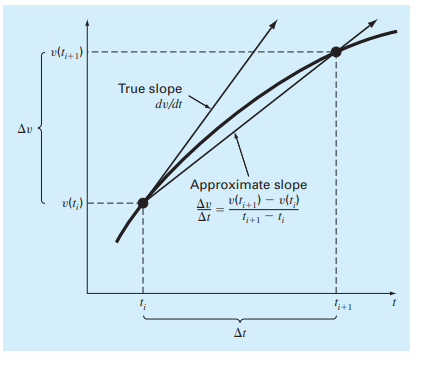
\includegraphics[width=0.75\textwidth]{fig_1_3}
   \caption{\textsf{The use of a finite difference to approximate the first derivative of v with respect to t.}}
   \label{fig:fig_1_3}
\end{figure}

Equation (1.11) is called a finite-difference approximation of the derivative at time ti .
It can be substituted into Eq. (1.8) to give

$$\dfrac{v(t_{i+1})-v(t_i)}{t_{i+1}-t_i}= g- \dfrac{c_d}{m}v(t_i)^2$$

This equation can then be rearranged to yield

\begin{equation}
	\tag{1.12}
	v(t_{i+1})= v(t_i)+ \left[ g- \dfrac{c_d}{m}v(t_i)^2 \right](t_{i+1}-t_i)
\end{equation}

Notice that the term in brackets is the right-hand side of the differential equation itself
[Eq. (1.8)]. That is, it provides a means to compute the rate of change or slope of v. Thus,
the equation can be rewritten more concisely as

\begin{equation}
	\tag{1.13}
	v_{i+1}=v_i + \dfrac{dv_i}{dt}\Delta t
\end{equation}

where the nomenclature $v_i$ designates velocity at time $t_i$ and $\Delta t = t_{i+1} − t_i$ .
We can now see that the differential equation has been transformed into an equation that
can be used to determine the velocity algebraically at $t_{i+1}$ using the slope and previous values
 of $v $and $t$. If you are given an initial value for velocity at some time ti, you can easily compute
  velocity at a later time$ t_{i+1}$. This new value of velocity at $ t_{i+1}$ can in turn be employed to
extend the computation to velocity at $t_{i+2} $and so on. Thus at any time along the way,

$$ New \ value = old \ value + slope \ \times  \ step \ size $$

This approach is formally called \textsl{uler's method}. We'll discuss it in more detail when we
turn to differential equations later in this book.


\section*{EXAMPLE 1.2. Numerical Solution to the Bungee Jumper Problem}

roblem Statement. Perform the same computation as in Example 1.1 but use Eq. (1.12)
to compute velocity with Euler's method. Employ a step size of 2 s for the calculation.

Solution. At the start of the computation $(t0 = 0)$, the velocity of the jumper is zero.
Using this information and the parameter values from Example 1.1, Eq. (1.12) can be used
to compute velocity at $t_1$ = 2 s:

$$ v= 0 \left[ 9.81 - \dfrac{0.25}{68.1}(0)^2 \right] \times 2 = 19.62 m/s$$ 

For the next interval (from $t$ = 2 to 4 s), the computation is repeated, with the result

$$ v= 19.62 \left[ 9.81 - \dfrac{0.25}{68.1}(19.62)^2 \right] \times 2 = 36.4137 m/s$$ 

\begin{figure}[H]
	\centering
	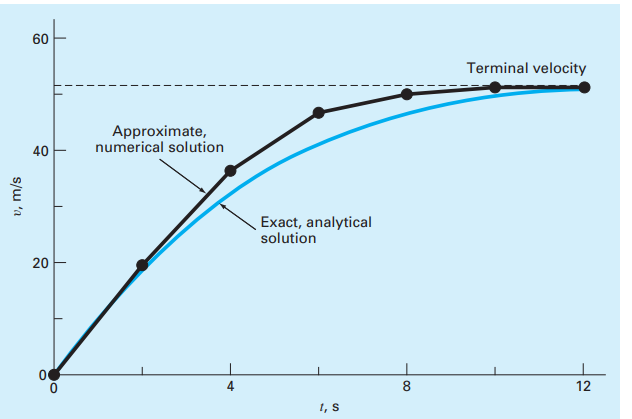
\includegraphics[width=0.75\textwidth]{fig_1_4}
   \caption{\textsf{Comparison of the numerical and analytical solutions for the bungee jumper problem.}}
   \label{fig_1.4}
\end{figure}


The calculation is continued in a similar fashion to obtain additional values:


\begin{table}[H]
	\begin{tabular}{c c}
		\hline
		\textbf{t,s} & \textbf{v, m/s} \\ 
		\hline
			0 &0\\
			2 &19.6200\\
			4 &36.4137\\
			6& 46.2983\\
			8 &50.1802\\
			10 & 51.3123\\
			12& 51.6008\\
			$\inf$ &51.6938 \\
			\hline
		
	\end{tabular}
\end{table}


The results are plotted in Fig. 1.4 along with the exact solution. We can see that the numerical method captures the essential features of the exact solution. However, because we
have employed straight-line segments to approximate a continuously curving function,
there is some discrepancy between the two results. One way to minimize such discrepancies is to use a smaller step size. For example, applying Eq. (1.12) at 1-s intervals results in
a smaller error, as the straight-line segments track closer to the true solution. Using hand
calculations, the effort associated with using smaller and smaller step sizes would make
such numerical solutions impractical. However, with the aid of the computer, large numbers of calculations can be performed easily. Thus, you can accurately model the velocity
of the jumper without having to solve the differential equation exactly. As in Example 1.2, a computational price must be paid for a more accurate numerical
result. Each halving of the step size to attain more accuracy leads to a doubling of the number of computations. Thus, we see that there is a trade-off between accuracy and computational effort. Such trade-offs figure prominently in numerical methods and constitute an
important theme of this book. 


\section {CONSERVATION LAWS IN ENGINEERING AND SCIENCE}

Aside from Newton's second law, there are other major organizing principles in science
and engineering. Among the most important of these are the conservation laws. Although
they form the basis for a variety of complicated and powerful mathematical models, the
great conservation laws of science and engineering are conceptually easy to understand.
They all boil down to

\begin{equation}
	\tag{1.14}
	Change\ = \ increases \ − \ decreases
\end{equation}

This is precisely the format that we employed when using Newton's law to develop a force
balance for the bungee jumper [Eq. (1.8)].

Although simple, Eq. (1.14) embodies one of the most fundamental ways in which
conservation laws are used in engineering and science-that is, to predict changes
with respect to time. We will give it a special name-the \textsl{time-variable (or transient)}
computation.

$$ Change =  0  =  increases  −  decreases $$

or

\begin{equation}
	\tag{1.15}
	Increases \ = \ decreases
\end{equation}

Thus, if no change occurs, the increases and decreases must be in balance. This case, which
is also given a special name-the steady-state calculation-has many applications in engineering and science. For example, for steady-state incompressible fluid flow in pipes, the
flow into a junction must be balanced by flow going out, as in

\begin{equation}
	Flow \ in = o \ w \ out
\end{equation}

For the junction in Fig. 1.5, the balance can be used to compute that the flow out of the
fourth pipe must be 60.

For the bungee jumper, the steady-state condition would correspond to the case where
the net force was zero or [Eq. (1.8) with $dv/dt = 0$]

\begin{equation}
	mg =c_dv^2
\end{equation}

Thus, at steady state, the downward and upward forces are in balance and Eq. (1.16) can be
solved for the terminal velocity


$$v=\sqrt{\dfrac{gm}{c_d}}  $$

Although Eqs. (1.14) and (1.15) might appear trivially simple, they embody the two fundamental ways that conservation laws are employed in engineering and science. As such, they
will form an important part of our efforts in subsequent chapters to illustrate the connection
between numerical methods and engineering and science.


\begin{figure}[H]
	\centering
	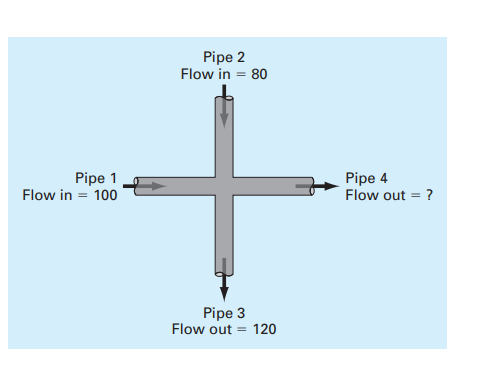
\includegraphics[width=0.75\textwidth]{fig_1_5}
   \caption{\textsf{A flow balance for steady incompressible fluid flow at the junction of pipes.}}
   \label{fig_1.5}
\end{figure}

Table 1.1 summarizes some models and associated conservation laws that figure prominently in engineering. Many chemical engineering problems involve mass balances for
reactors. The mass balance is derived from the conservation of mass. It specifies that the
change of mass of a chemical in the reactor depends on the amount of mass flowing in
minus the mass flowing out.

Civil and mechanical engineers often focus on models developed from the conservation of momentum. For civil engineering, force balances are utilized to analyze structures
such as the simple truss in Table 1.1. The same principles are employed for the mechanical
engineering case studies to analyze the transient up-and-down motion or vibrations of an
automobile.

Finally, electrical engineering studies employ both current and energy balances to model
electric circuits. The current balance, which results from the conservation of charge, is similar in 
spirit to the flow balance depicted in Fig. 1.5. Just as flow must balance at the junction
of pipes, electric current must balance at the junction of electric wires. The energy balance
specifies that the changes of voltage around any loop of the circuit must add up to zero.



\section{NUMERICAL METHODS COVERED IN THIS BOOK}

Euler's method was chosen for this introductory chapter because it is typical of many other
classes of numerical methods. In essence, most consist of recasting mathematical operations 
into the simple kind of algebraic and logical operations compatible with digital computers.
 Figure 1.6 summarizes the major areas covered in this text. 
\begin{table}[H]
\caption{\textsf{Devices and types of balances that are commonly used in the four major areas of engineering. For
each case, the conservation law on which the balance is based is specified.}}
 \begin{figure}[H]
	\centering
	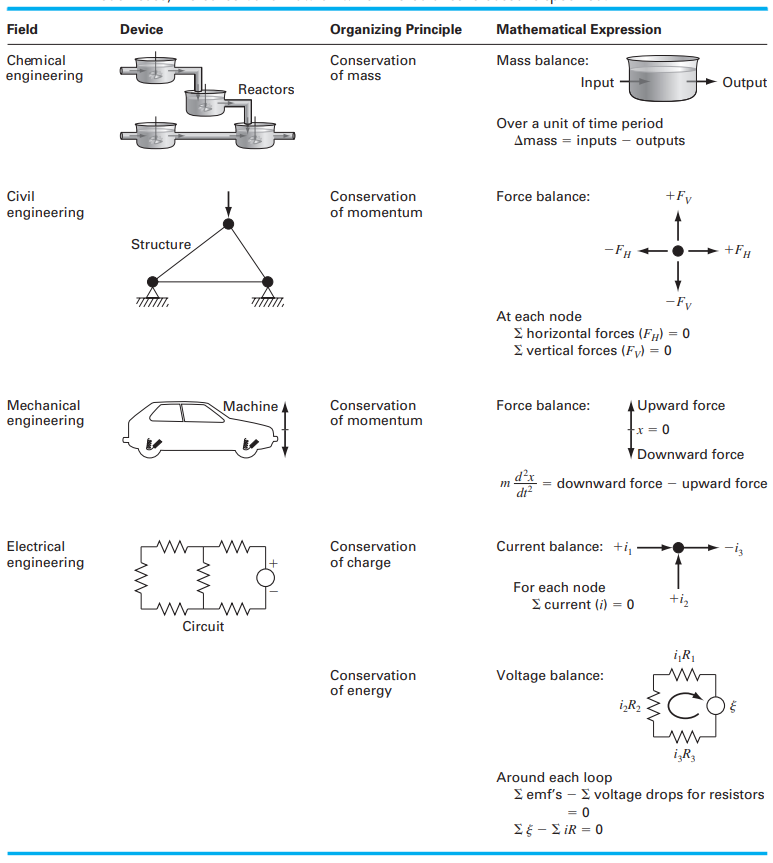
\includegraphics[width=1\textwidth]{fig_1_4t}
   
   \label{fig_1.}
\end{figure}
\end{table}


\begin{figure}[H]
	\centering
	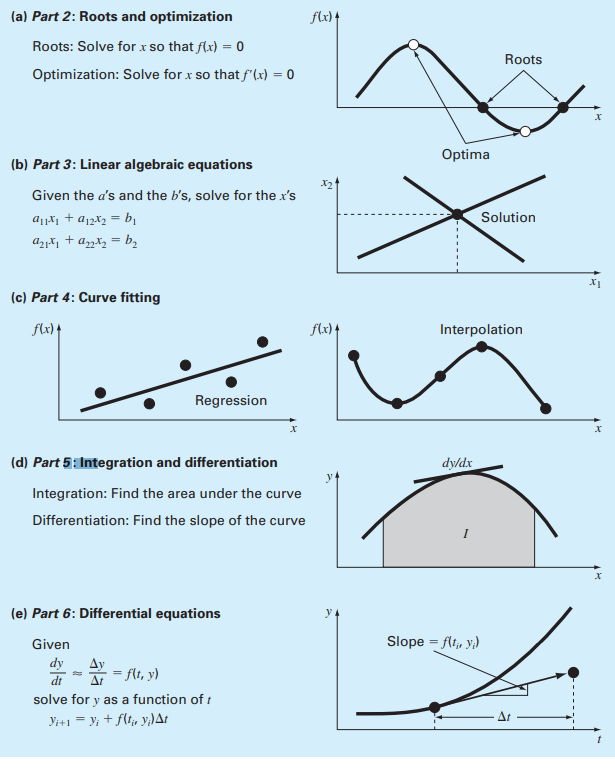
\includegraphics[width=0.8\textwidth]{fig_1_6}
   \caption{\textsf{Summary of the numerical methods covered in this book.}}
   \label{fig_1.}
\end{figure}


Part Two deals with two related topics: root finding and optimization. As depicted in
Fig. 1.6a, root location involves searching for the zeros of a function. In contrast, optimization involves determining 
a value or values of an independent variable that correspond to a
"best" or optimal value of a function. Thus, as in Fig. 1.6a, optimization involves identifying maxima and minima.
 Although somewhat different approaches are used, root location
and optimization both typically arise in design contexts.

Part Three is devoted to solving systems of simultaneous linear algebraic equations
(Fig. 1.6b). Such systems are similar in spirit to roots of equations in the sense that they are
concerned with values that satisfy equations. However, in contrast to satisfying a single
equation, a set of values is sought that simultaneously satisfies a set of linear algebraic
equations. Such equations arise in a variety of problem contexts and in all disciplines of engineering and 
science. In particular, they originate in the mathematical modeling of large
systems of interconnected elements such as structures, electric circuits, and fluid networks.
However, they are also encountered in other areas of numerical methods such as curve fitting and differential equations.


As an engineer or scientist, you will often have occasion to fit curves to data points.
The techniques developed for this purpose can be divided into two general categories:
regression and interpolation. As described in Part Four (Fig. 1.6c), regression is
employed where there is a significant degree of error associated with the data. Experimental results are often of this kind. For these situations, the strategy is to derive a single curve that represents the general trend of the data without necessarily matching any
individual points.

In contrast, interpolation is used where the objective is to determine intermediate values between relatively error-free data points. Such is usually the case for tabulated information. The strategy in such cases is to fit a curve directly through the data points and use
the curve to predict the intermediate values.


As depicted in Fig. 1.6d, Part Five is devoted to integration and differentiation. A
physical interpretation of numerical integration is the determination of the area under a
curve. Integration has many applications in engineering and science, ranging from the
determination of the centroids of oddly shaped objects to the calculation of total quantities based on sets 
of discrete measurements. In addition, numerical integration formulas play an important role in the solution of 
differential equations. Part Five also covers
methods for numerical differentiation. As you know from your study of calculus, this
involves the determination of a function's slope or its rate of change.


Finally, Part Six focuses on the solution of ordinary differential equations (Fig. 1.6e).
Such equations are of great significance in all areas of engineering and science. This is
because many physical laws are couched in terms of the rate of change of a quantity rather
than the magnitude of the quantity itself. Examples range from population-forecasting
models (rate of change of population) to the acceleration of a falling body (rate of change
of velocity). Two types of problems are addressed: initial-value and boundary-value
problems.

\section*{\textbf{CASE STUDY} IT'S A REAL DRAG}

\textbf{Background}. In our model of the free-falling bungee jumper, we assumed that drag
depends on the square of velocity (Eq. 1.7). A more detailed representation, which was
originally formulated by Lord Rayleigh, can be written as

\begin{equation}
	\tag{1.17}
	F_d =-\dfrac{1}{2}\rho v^2AC_d\overrightarrow{v} 
\end{equation}

where $F_d$  the drag force (N),$\rho$   fluid density ($kg/m^3$), A \= the frontal area of the object
on a plane perpendicular to the direction of motion ($m^2$), $C_d$  a dimensionless drag coefficient, 
and $\overrightarrow{v}$  \=  a unit vector indicating the direction of velocity.


This relationship, which assumes turbulent conditions (i.e., a high Reynolds number),
allows us to express the lumped drag coefficient from Eq. (1.7) in more fundamental terms
as
\begin{equation}
	\tag{1.18}
	C_d=\dfrac{1}{2}\rho AC_d
\end{equation}

Thus, the lumped drag coefficient depends on the object's area, the fluid's density, and a
dimensionless drag coefficient. The latter accounts for all the other factors that contribute
to air resistance such as the object's "roughness". For example, a jumper wearing a baggy
outfit will have a higher $C_d$ than one wearing a sleek jumpsuit.

Note that for cases where velocity is very low, the flow regime around the object will
be laminar and the relationship between the drag force and velocity becomes linear. This is
referred to as \textsl{Stokes drag}.

In developing our bungee jumper model, we assumed that the downward direction was
positive. Thus, Eq. (1.7) is an accurate representation of Eq. (1.17), because $\overrightarrow{v} + 1$    and
the drag force is negative. Hence, drag reduces velocity.


But what happens if the jumper has an upward (i.e., negative) velocity? In this case,
$\overrightarrow{v} –1$ and Eq. (1.17) yields a positive drag force. Again, this is physically correct as the positive 
drag force acts downward against the upward negative velocity.


Unfortunately, for this case, Eq. (1.7) yields a negative drag force because it does not
include the unit directional vector. In other words, by squaring the velocity, its sign and
hence its direction is lost. Consequently, the model yields the physically unrealistic result
that air resistance acts to accelerate an upward velocity!


In this case study, we will modify our model so that it works properly for both downward
and upward velocities. We will test the modified model for the same case as Example 1.2, but
with an initial value of $v(0)$ = -40 m/s. In addition, we will  also illustrate how we can extend
the numerical analysis to determine the jumper's position.


Solution. The following simple modification allows the sign to be incorporated into
the drag force:

\begin{equation}
	\tag{1.19}
	F_d=-\dfrac{1}{2}\rho v|v|AC_d
\end{equation}

or in terms of the lumped drag:

\begin{equation}
	\tag{1.20}
	F_d=-c_dV|v|
\end{equation}

Thus, the differential equation to be solved is

\begin{equation}
	\tag{1.21}
	\dfrac{dv}{dt}= g - \dfrac{c_d}{m}v|v|
\end{equation}

In order to determine the jumper's position, we recognize that distance travelled,
x (m), is related to velocity by


\begin{equation}
	\tag{1.22}
	\dfrac{dv}{dt}= -v
\end{equation}

In contrast to velocity, this formulation assumes that upward distance is positive. In the
same fashion as Eq. (1.12), this equation can be integrated numerically with Euler's
method:

\begin{equation}
	\tag{1.23}
	x-{i+1}=x_i-v(t_i)\Delta t
\end{equation}

Assuming that the jumper's initial position is defined as x(0)  0, and using the parameter values
 from Examples 1.1 and 1.2, the velocity and distance at t  2 s can be computed as

$$v(2)= -40 + \left[ 9.81 - \dfrac{0.25}{68.1}(-40)(40) \right]2= -8.6326 m/s $$
$$x(2)=0 - (-40)2=80 m$$

 Note that if we had used the incorrect drag formulation, the results would be 32.1274 m/s
and 80 m. 

The computation can be repeated for the next interval (t  2 to 4 s):

$$v(2)= -8.6326 + \left[ 9.81 - \dfrac{0.25}{68.1}(-8.6326)(8.6326) \right]2= 11.5346 m/s $$
$$x(4) =80 -(-8.6326)2=97.27651 m $$


The incorrect drag formulation gives –20.0858 m/s and 144.2549 m.


The calculation is continued and the results shown in Fig. 1.7 along with those
obtained with the incorrect drag model. Notice that the correct formulation decelerates
more rapidly because drag always diminishes the velocity.


With time, both velocity solutions converge on the same terminal velocity because
eventually both are directed downward in which case, Eq. (1.7) is correct. However, the
impact on the height prediction is quite dramatic with the incorrect drag case resulting in a
much higher trajectory.


This case study demonstrates how important it is to have the correct physical model.
In some cases, the solution will yield results that are clearly unrealistic. The current example is more insidious as there is no visual evidence that the incorrect solution is wrong. That
is, the incorrect solution “looks” reasonable.

\begin{figure}[H]
	\centering
	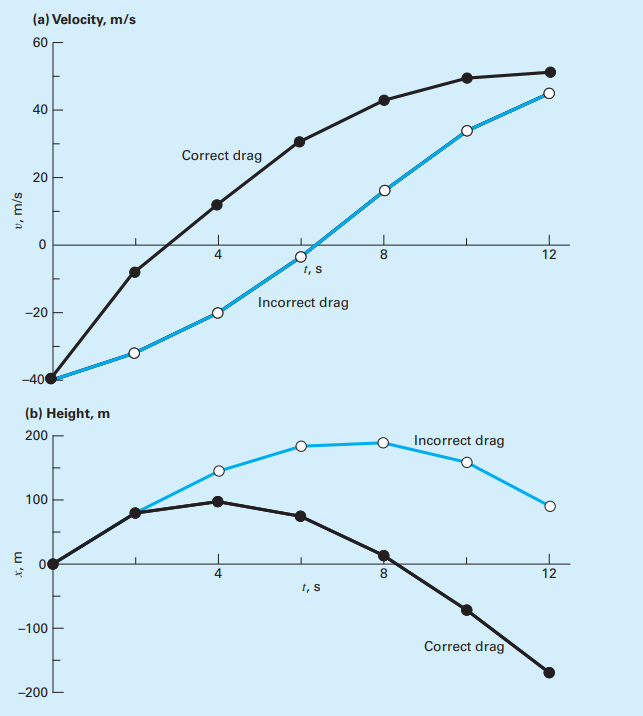
\includegraphics[width=0.80\textwidth]{fig_1_7}
   \caption{\textsf{Plots of (a) velocity and (b) height for the free-falling bungee jumper with an upward (negative)
   initial velocity generated with Euler's method. Results for both the correct (Eq. 1 20) and incorrect
   (Eq. 1.7) drag formulations are displayed.}}
   \label{fig_1.}
\end{figure}

\section*{problems}

\begin{multicols}{2}
	
	\textbf{1.1} Use calculus to verify that Eq. (1.9) is a solution of
Eq. (1.8) for the initial condition v(0)  0.


\textbf{1.2} Use calculus to solve Eq. (1.21) for the case where the initial velocity is (a) positive and (b) negative. (c) Based on your
results for (a) and (b), perform the same computation as in Example 1.1 but with an initial velocity of -40 m/s. Compute
values of the velocity from t  0 to 12 s at intervals of 2 s. Note
that for this case, the zero velocity occurs at t  3.470239 s.


\textbf{1.3} The following information is available for a bank account:

\begin{table}[H]
	
		\begin{tabular}{cccc }
			\hline
			Date &Deposits& Withdrawals &Balance\\
			\hline
			5/1&&& 1512.33\\
			&220.13& 327.26&\\
			6/1&&&\\
			&216.80& 378.61&\\
			7/1&&&\\
			&450.25 &106.80&\\
			8/1&&&\\
			&127.31 &350.61&\\
			9/1&&&\\
			\hline
		\end{tabular}
\end{table}

Note that the money earns interest which is computed as
$$Interest = i B_i $$

where i  the interest rate expressed as a fraction per month,
and $B_i$ the initial balance at the beginning of the month.
\begin{enumerate}[label=(\alph*)]
	\item Use the conservation of cash to compute the balance on
	6/1, 7/1, 8/1, and 9/1 if the interest rate is 1\% per month
	($i =  0.01/month$). Show each step in the computation
	\item Write a differential equation for the cash balance in the
	form

	$$\dfrac{dB}{dt}=f[D(t), W(t), i  ]$$

	where t  time (months), D(t)  deposits as a function
of time (\$\/month), W(t)  withdrawals as a function of
time (\$\/month). For this case, assume that interest  is
compounded continuously; that is, interest  =$iB$

\item Use Euler's method with a time step of 0.5 month to
simulate the balance. Assume that the deposits and withdrawals are applied uniformly over the month. 
\item Develop a plot of balance versus time for (a) and (c).
\end{enumerate}


\textbf{1.4} Repeat Example 1.2. Compute the velocity to $t = 12 s$,
with a step size of (a) 1 and (b) 0.5 s. Can you make any
statement regarding the errors of the calculation based on the
results?

\textbf{1.5} Rather than the nonlinear relationship of Eq. (1.7), you
might choose to model the upward force on the bungee
jumper as a linear relationship:

$$F_U = -c'v$$

where c' = a first-order drag coefficient (kg/s). 
\begin{enumerate}[label=(\alph*)]
	\item Using calculus, obtain the closed-form solution for the
	case where the jumper is initially at rest ($v = 0 at t = 0$)
	\item Repeat the numerical calculation in Example 1.2 with
	the same initial condition and parameter values. Use a
	value of 11.5 kg/s for c'.
\end{enumerate}

\textbf{1.6} For the free-falling bungee jumper with linear drag
(Prob. 1.5), assume a first jumper is 70 kg and has a drag coefficient of 12 kg/s. If a second jumper has a drag coefficient
of 15 kg/s and a mass of 80 kg, how long will it take her to
reach the same velocity jumper 1 reached in 9 s?


\textbf{1.7} For the second-order drag model (Eq. 1.8), compute the
velocity of a free-falling parachutist using Euler's method
for the case where $m = 80 kg$ and $c_d = 0.25 kg/m$. Perform
the calculation from $t = 0$ to $20 s$ with a step size of 1 s. Use
an initial condition that the parachutist has an upward velocity of 
20 m/s at t = 0. At $t = 10 s$, assume that the chute is
instantaneously deployed so that the drag coefficient jumps
to 1.5 kg/m.

\textbf{1.8} The amount of a uniformly distributed radioactive contaminant contained in a closed reactor is measured by its
concentration c (becquerel/liter or Bq/L). The contaminant
decreases at a decay rate proportional to its concentration;
that is

$$ Decay\ rate =  -kc $$

where k is a constant with units of $day^{-1}$
. Therefore, according to Eq. (1.14), a mass balance for the reactor can be
written as

\[ \begin{array}{c c c}
	\dfrac{dc}{dt} & =& -kc\\
	\binom{change}{in \ mass} & =& \binom{decrease}{by \ decay} 
	
\end{array} \]

\begin{enumerate}[label=(\alph*)]
	\item Use Euler's method to solve this equation from $t$ \= 0 to
	1 d with $k$ \= 0.175 $d^-1$. Employ a step size of $\Delta t$ \= 0.1 d.
	The concentration at $t$ \= 0 is 100 Bq/L.
	\item Plot the solution on a semilog graph (i.e., ln $c$ versus $t$)
	and determine the slope. Interpret your results
\end{enumerate}

\textbf{1.9} A storage tank (Fig. P1.9) contains a liquid at depth y
where y = 0 when the tank is half full. Liquid is withdrawn
at a constant flow rate Q to meet demands. The contents are


\begin{figure}[H]
	\centering
	
	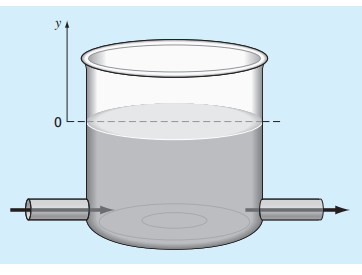
\includegraphics[width=0.45\textwidth]{fig_P1_9}
	\caption*{Figure P1.9}
   \label{fig_P1.9}
\end{figure}

resupplied at a sinusoidal rate $3Q$ $sin^2(t)$. Equation (1.14)
can be written for this system as

$$ \dfrac{d(Ay)}{dt}=3Q sin^2(t)-Q$$
$$ \binom{change \ in}{volume} = (in \ o \ w) - (out \ o \ w) $$

or, since the surface area A is constant

$$\dfrac{dy}{dt}=3\dfrac{Q}{A}sin^2(t)- \dfrac{\alpha(1+y)^{1.5}}{A} $$

Use Euler's method to solve for the depth y from $t = 0$ to
10 d with a step size of 0.5 d. The parameter values are $A =
1250 m^2$, $Q = 450 m^3/d$, and $\alpha = 150$. Assume that the initial condition is $y = 0$.

\textbf1.11 Apply the conservation of volume (see Prob. 1.9) to simulate the level of liquid in a conical storage tank (Fig. P1.11).

\begin{figure}[H]
	\centering
	
	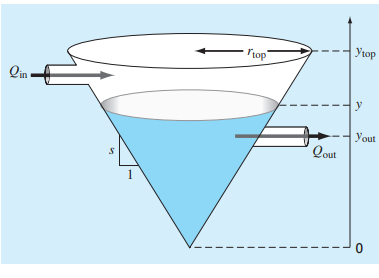
\includegraphics[width=0.45\textwidth]{fig_P1_11}
	\caption*{Figure P1.11}
   \label{fig_P1.9}
\end{figure}

The liquid flows in at a sinusoidal rate of $Q_{in} = 3 sin^2
(t)$ and
flows out according to

\[\begin{array}{r c l  r c l}
	Q_{out}& =& 3(y − yout)^{1.5} & y &>& yout\\
	Q_{out}& =& 0& y& \leq  &yout\\

	
\end{array} \]

where flow has units of $m^3/d$ and $y =$ the elevation of the
water surface above the bottom of the tank (m). Use Euler's
method to solve for the depth y from $t = 0$ to 10 d with a step
size of 0.5 d. The parameter values are $r_top$  2.5 m, $y_top$  4 m,
and $y_out$  1 m. Assume that the level is initially below the
outlet pipe with $y(0)$  0.8 m


\textbf{1.12} A group of 35 students attend a class in an insulated
room which measures 11 m by 8 m by 3 m. Each student
takes up about $0.075 m^3$ and gives out about 80 W of heat
(1 W = 1 J/s). Calculate the air temperature rise during the first
20 minutes of the class if the room is completely sealed and insulated. 
Assume the heat capacity $C_v$ for air is 0.718 kJ/(kg K).
Assume air is an ideal gas at 20°C and 101.325 kPa. Note
that the heat absorbed by the air Q is related to the mass of
the air m the heat capacity, and the change in temperature by
the following relationship:

$$Q= m \int_{T_2}^{T_1}  C_v\,dT =mC_v(T_2-T_1) $$

The mass of air can be obtained from the ideal gas law:

$$PV= \dfrac{m}{Mwt}RT$$

where P is the gas pressure, V is the volume of the gas, Mwt
is the molecular weight of the gas (for air, 28.97 kg/kmol),
and $R$ is the ideal gas constant [8.314 kPa $m^3$
/(kmol K)].

\begin{figure}[H]
	\centering
	
	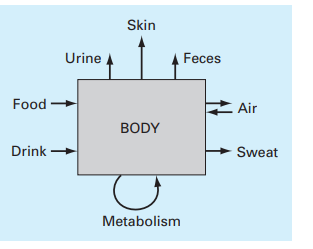
\includegraphics[width=0.45\textwidth]{fig_P1_13}
	\caption*{Figure P1.13}
   \label{fig_1.}
\end{figure}

\textbf{1.13} Figure P1.13 depicts the various ways in which an average man gains and loses water in one day. One liter is ingested
as food, and the body metabolically produces 0.3 liters. In
breathing air, the exchange is 0.05 liters while inhaling, and
0.4 liters while exhaling over a one-day period. The body will
also lose 0.3, 1.4, 0.2, and 0.35 liters through sweat, urine,
feces, and through the skin, respectively. To maintain steady
state, how much water must be drunk per day?

\textbf{1.14} In our example of the free-falling bungee jumper, we
assumed that the acceleration due to gravity was a constant
value of 9.81 $m/s^2$
. Although this is a decent approximation
when we are examining falling objects near the surface of
the earth, the gravitational force decreases as we move
above sea level. A more general representation based on
Newton's inverse square law of gravitational attraction can
be written as

$$ g(x)= g(0)\dfrac{R^2}{(R+x)^2}$$

where g(x) = gravitational acceleration at altitude $x$ (in m)
measured upward from the earth's surface $(m/s^2), g(0) =$
gravitational acceleration at the earth's surface ($\cong  9.81 m/s^2)$,
and $R =$ the earth's radius ($\cong  6.37 × 10^6 m$). 
\begin{enumerate}[label=(\alph*)]
	\item  In a fashion similar to the derivation of Eq. (1.8), use a
	force balance to derive a differential equation for velocity as a function of time that utilizes this more complete
	representation of gravitation. However, for this derivation, assume that upward velocity is positive. 

	\item For the case where drag is negligible, use the chain rule
	to express the differential equation as a function of altitude rather than time. Recall that the chain rule is

	$$\dfrac{dv}{dt} = \dfrac{dv}{dx}\dfrac{dx}{dt} $$

	\item Use calculus to obtain the closed form solution where
	$$ v=v_0 \text{at} x=0 $$
	\item Use Euler's method to obtain a numerical solution from
	x = 0 to 100,000 m using a step of 10,000 m where the
	initial velocity is 1500 m/s upward. Compare your result
	with the analytical solution.


\end{enumerate}

\textbf{1.15} Suppose that a spherical droplet of liquid evaporates at
a rate that is proportional to its surface area.


$$ \dfrac{dV}{dt} = -kA$$

where $V =$ volume ($mm^3$), $t =$ time (min), $k =$ the evaporation rate (mm/min), and $A =$ surface area ($mm^2$). Use
Euler's method to compute the volume of the droplet from
$t =$ 0 to 10 min using a step size of 0.25 min. Assume that
$k =$ 0.08 mm/min and that the droplet initially has a radius of
2.5 mm. Assess the validity of your results by determining
the radius of your final computed volume and verifying that
it is consistent with the evaporation rate. 

\textbf{1.16} A fluid is pumped into the network shown in Fig. P1.16.
If $Q_2 = 0.7, Q_3 = 0.5, Q_7 = 0.1$, and $Q8 = 0.3 m^3/s$, determine
the other flows


\textbf{1.17} Newton's law of cooling says that the temperature of a
body changes at a rate proportional to the difference between
its temperature and that of the surrounding medium (the ambient temperature),
\begin{figure}[H]
	\centering
	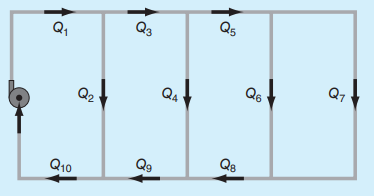
\includegraphics[width=0.45\textwidth]{fig_P1_16}
   \caption*{Figure P1.16}
   \label{fig_1.}
\end{figure}

$$\dfrac{dT}{dt}= -k(T -T_aa)$$

where $T =$ the temperature of the body (°C), $t =$ time (min),
$k =$ the proportionality constant (per minute), and $T_a =$ the
ambient temperature (°C). Suppose that a cup of coffee originally has a temperature of 70 °C. Use Euler's method to
compute the temperature from $t =$ 0 to 20 min using a step
size of 2 min if $T_a =$ 20 °C and $k =$ 0.019/min.

\textbf{1.18} You are working as a crime scene investigator and
must predict the temperature of a homicide victim over a
5-hour period. You know that the room where the victim was
found was at 10 °C when the body was discovered.
\begin{enumerate}[label=(\alph*)]
	\item Use Newton's law of cooling (Prob. 1.17) and Euler's
	method to compute the victim's body temperature for
	the 5-hr period using values of $k=$  0.12/hr and $\Delta t$
	0.5 hr. Assume that the victim's body temperature at
	the time of death was 37 °C, and that the room temperature was at a constant value of 10 °C over the 5-hr
	period.
	\item Further investigation reveals that the room temperature
	had actually dropped linearly from 20 to 10 °C over the
	5-hr period. Repeat the same calculation as in (a) but incorporate this new information
	\item Compare the results from (a) and (b) by plotting them
	on the same graph. 
\end{enumerate}

\textbf1.19 The velocity is equal to the rate of change of distance,
x(m):
$$\dfrac{dx}{dt} = v(t)$$


Use Euler's method to numerically integrate Eq. (P1.19) and
(1.8) in order to determine both the velocity and distance
fallen as a function of time for the first 10 seconds of freefall
using the same parameters and conditions as in Example 1.2.
Develop a plot of your results.

\textbf{1.20} In addition to the downward force of gravity (weight)
and drag, an object falling through a fluid is also subject to a
buoyancy force which is proportional to the displaced volume. For example, for a sphere with diameter $d (m)$, the
sphere's volume is$ V  \pi  d^3/6$, and its projected area isA  $\pi ^2/4$. The buoyancy force can then be computed as
$F_b= -\rho Vg$. We neglected buoyancy in our derivation of
Eq. (1.8) because it is relatively small for an object like a
bungee jumper moving through air. However, for a more
dense fluid like water, it becomes more prominent.
\begin{enumerate}[label=(\alph*)]
	\item Derive a differential equation in the same fashion as
	Eq. (1.8), but include the buoyancy force and represent
	the drag force as described in Sec. 1.4.
	\item Rewrite the differential equation from (a) for the special
	case of a sphere.
	\item Use the equation developed in (b) to compute the terminal
	velocity (i.e., for the steady-state case). Use the following
	parameter values for a sphere falling through water:
	sphere diameter  1 cm, sphere density  2,700 $kg/m^3$,
	water density  1,000 $kg/m^3$, and $C_d$  0.47.
	\item Use Euler's method with a step size of $\Delta t $ 0.03125 s to
	numerically solve for the velocity from t  0 to 0.25 s
	with an initial velocity of zero. 
	
\end{enumerate}

\end{multicols}

\end{document}


\begin{table}[H]
	\caption{Tablica ilorazów różnicowych}
		\begin{tabular}{|c| c|c| c|c| c|c| }
			\hline 

			&&&&


			\begin{figure}[H]
				\centering
				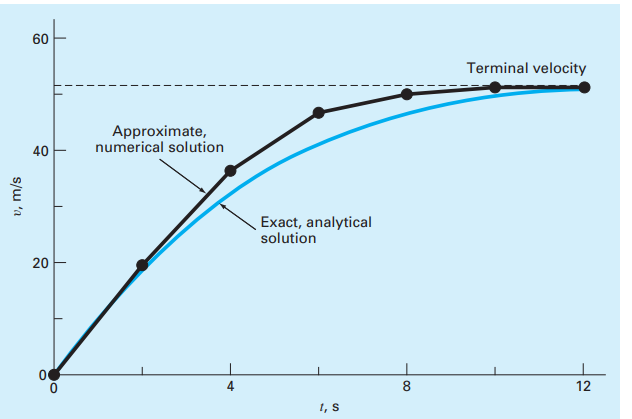
\includegraphics[width=0.75\textwidth]{fig_1_4}
			   \caption{\textsf{Comparison of the numerical and analytical solutions for the bungee jumper problem.}}
			   \label{fig_1.}
			\end{figure}


